\documentclass[10pt]{article}
\usepackage[margin=0.8in]{geometry}
\usepackage[T1]{fontenc}
\usepackage{lmodern,booktabs,graphicx,longtable,hyperref}
\title{Supplement S1b: Endpoint robustness}
\author{Anonymous authors}
\date{}
\begin{document}\maketitle
\section{Scope and reproducibility}
The data are the same 658 R2 TEST participants and 49 endpoints used previously. No inference, new participant recruitment or model fitting occurred. Analyses were specified after prior R2 outcomes were known and are exploratory, not external preregistration. Participant-level losses remain in restricted storage; only aggregate outputs are included here.

The seven contrasts, weighting schemes and seed were fixed in SPEC.md before execution. The frozen CAL denominators, mixture weights and statistical decoders were unchanged. Uncertainty uses the same 10,000 paired participant samples across contrasts. The alternative aggregation does not replace the original primary target or its multiplicity decisions. Endpoint omission removes one endpoint and re-normalizes only the weights within the original families. It is a sensitivity of point estimates, not inference over a new task distribution.

Source, audit-receipt and verifier SHA256 checks run before loading; original Granite-versus-Full1400 point estimates are recovered to absolute tolerance $10^{-12}$. A separate local arithmetic audit reconstructed both aggregates and all 343 endpoint-omission estimates from exported endpoint means. This does not independently recompute bootstrap intervals from individual responses.
\section{Equal-family and equal-endpoint contrasts}
All differences are system minus reference. Lower favors the system. Intervals below are the new exploratory bootstrap intervals, including where the same original point estimate is reproduced. Registered intervals in the main text retain their original randomization and multiplicity analysis.
\begin{longtable}{@{}p{.31\textwidth}rr@{}}\toprule
System / reference & Equal family [95\% CI] & Equal endpoint [95\% CI]\\\midrule
Granite neutral / decoder1200 & -0.002886 [-0.004478, -0.001282] & -0.002980 [-0.004438, -0.001537]\\
Granite T0 / decoder1200 & -0.002689 [-0.004239, -0.001123] & -0.002550 [-0.003924, -0.001206]\\
Qwen neutral / decoder1200 & -0.000872 [-0.003070, +0.001314] & -0.001398 [-0.002819, -0.000042]\\
Qwen T0 / decoder1200 & +0.000050 [-0.001549, +0.001636] & -0.000960 [-0.002442, +0.000413]\\
Granite neutral / Full1400 & -0.004036 [-0.007178, -0.000932] & -0.003085 [-0.006059, -0.000087]\\
Granite T0 / Full1400 & -0.003839 [-0.006961, -0.000756] & -0.002654 [-0.005583, +0.000235]\\
Granite T0 / Granite neutral & +0.000197 [-0.000541, +0.000957] & +0.000431 [-0.000338, +0.001225]\\
\bottomrule\end{longtable}
\section{Separate families}
Economic preferences contains 40 pricing tasks. The heuristic/cognitive-bias family contains the other nine. Each table cell is normalized within the endpoint by its frozen CAL prior loss. Native endpoint RPS or log loss is retained in RESULT.json and must not be averaged across unlike loss scales.
\begin{longtable}{@{}p{.31\textwidth}rr@{}}\toprule
System / reference & Economic [95\% CI] & Other [95\% CI]\\\midrule
Granite neutral / decoder1200 & -0.003035 [-0.004708, -0.001360] & -0.002737 [-0.005520, +0.000044]\\
Granite T0 / decoder1200 & -0.002468 [-0.004032, -0.000940] & -0.002910 [-0.005704, -0.000150]\\
Qwen neutral / decoder1200 & -0.001703 [-0.003149, -0.000356] & -0.000042 [-0.004170, +0.004093]\\
Qwen T0 / decoder1200 & -0.001547 [-0.003257, +0.000034] & +0.001647 [-0.001108, +0.004384]\\
Granite neutral / Full1400 & -0.002533 [-0.006018, +0.000869] & -0.005538 [-0.010654, -0.000463]\\
Granite T0 / Full1400 & -0.001967 [-0.005396, +0.001331] & -0.005711 [-0.010895, -0.000603]\\
Granite T0 / Granite neutral & +0.000567 [-0.000341, +0.001499] & -0.000173 [-0.001318, +0.000996]\\
\bottomrule\end{longtable}
\begin{figure}[ht]\centering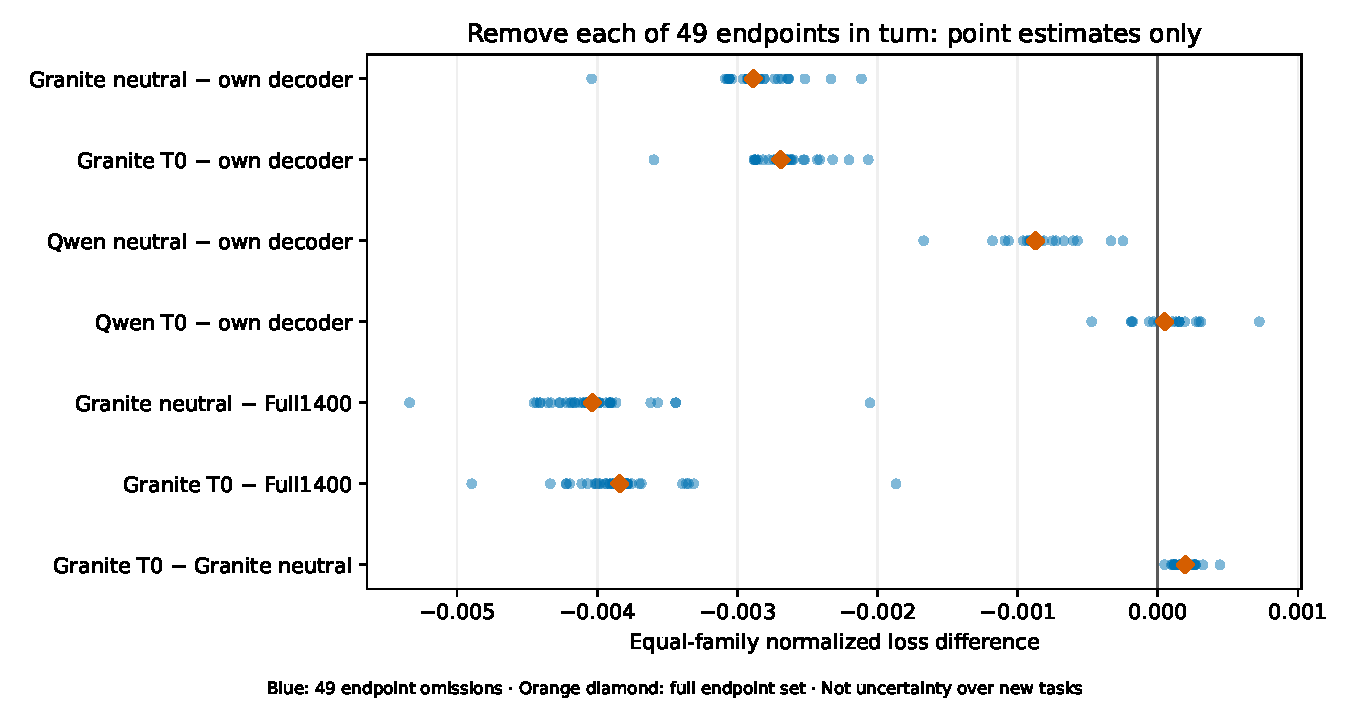
\includegraphics[width=\textwidth]{r2-endpoint-omission.pdf}\caption{All 49 omissions per contrast. Orange diamonds retain all endpoints. A retained negative point sign does not imply every omission has a statistically favorable interval.}\end{figure}
\section{Evidence chronology}
\begin{longtable}{@{}p{.16\textwidth}p{.76\textwidth}@{}}\toprule
Evidence & Interpretation\\\midrule
Original IPIP & Planned optimizer contrasts on fixed panels, followed by exploratory screens.\\
E1 & New same-corpus people for old templates; not new optimizer seeds.\\
E2 & Selector study on already exposed original outcomes.\\
E3 & Third same-corpus panel, frozen historical mixture recipes; broader historical supervision than its 80-person decoder fit.\\
B1/E4 & Reuse E3 for capacity, answer-budget and fixed-weight comparisons.\\
R2 & Frozen after an earlier CAL diagnostic, before its own fits/inference; public outcomes and unknown pretraining exposure.\\
Follow-ups & Reuse R2 TEST; post hoc, outside registered Holm family.\\
A17 & Planned independent panel; held, no new outcomes and no scientific result.\\\bottomrule
\end{longtable}
\section{Unresolved boundaries}
No analysis here estimates future optimizer-run uncertainty, new-task generalization, behavioral validity or acceptance probability. The candidate ACL paper and this supplement remain author-review drafts. Supplements S2--S4 retain the earlier methods and historical table numbering. Rights, anonymized release, publication overlap and final submission declarations require author resolution.
\end{document}
